\chapter{Results}
\label{results}

\textit{This section could be renamed to Numerical Examples, and
  should include any and all verification/validation work. To be
  clear, for the purpose of the SAND report, we don't require any
  validation. I will have to include a description of the Sierra input
  parameters for use in their user's manual, but obviously I'll worry
  about that.}

\section{Uniaxial Tension}
\label{tension}

In this section we investigate the behavior of the model in a state of
uniaxial tension. In particular, we will observe the stress and void
volume fraction response for a variety of failure parameter
combinations to develop an understanding of the behavior of the
model. Figure~\ref{tension-kw} shows the model behavior for various
values of the shear parameter $k_{\omega}$, and evidently it has
little to no effect on the response for this stress state.

\begin{figure}[htbp]
  \begin{center}
    \subfigure[stress]{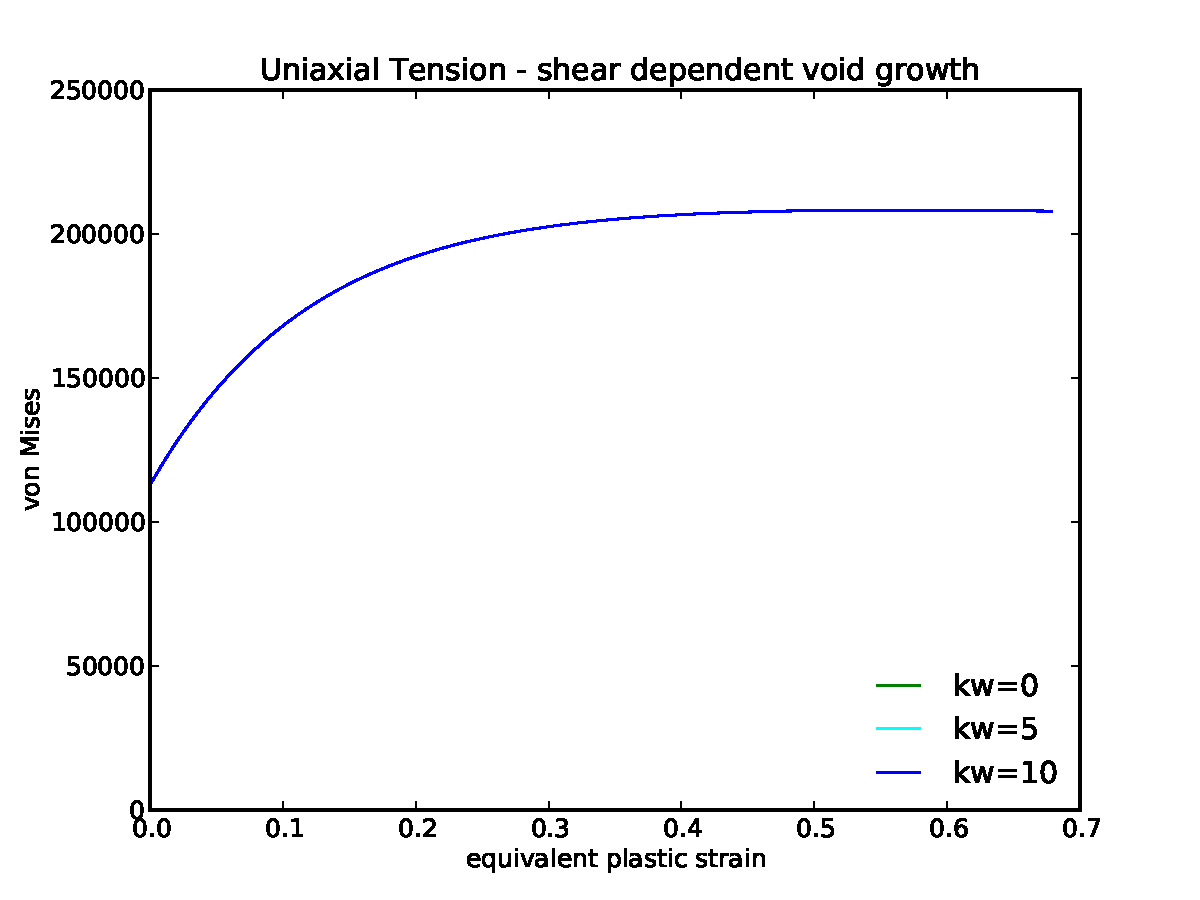
\includegraphics[trim=0mm 0mm 0mm 0
        mm,clip,width=0.5\textwidth]
      {images/stress-strain-tension-kw.pdf}}~ \subfigure[void volume
      fraction]{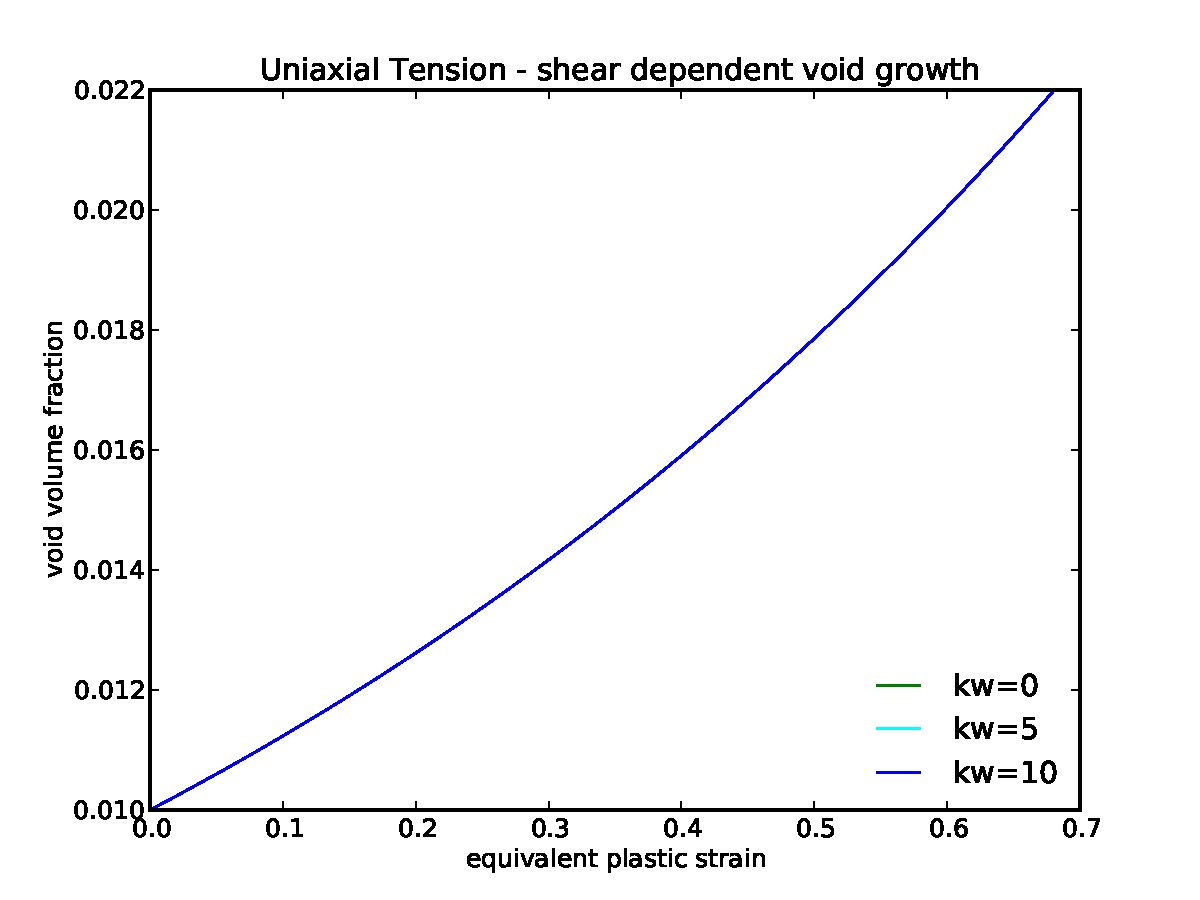
\includegraphics[trim=0mm 0mm 0mm 0
        mm,clip,width=0.5\textwidth]
      {images/void-strain-tension-kw.pdf}}
    \caption{Von Mises stress component and void volume fraction plotted
      against equivalent plastic strain. The shear void growth
      parameter has an insignificant effect on the response of the
      material point in tension.}
    \label{fig:tension-kw}
  \end{center}
\end{figure}

In Figure~\ref{fig:tension-nuc} a set of nucleation parameters are
specified and also evaluated in the uniaxial tension scenario. In this
case the volume fraction of nucleated voids $f_{N}$, is varied, while
the mean value and standard deviation of failure strain, $\epsilon_N$
and $s_N$ respectively, are specified and held constant. Observe that
the von Mises stress component is somewhat reduced, to a greater extent as
the volume fraction of nucleated voids is increased. Also observe that
the void volume fraction grows by approximately the specified volume
fraction of nucleated voids, accelerated the apparent void growth
until the total void volume fraction of nucleated void has been
exhausted. Afterwards, the trajectory returns to that of the void
growth without augmentation.

\begin{figure}[htbp]
  \begin{center}
    \subfigure[stress]{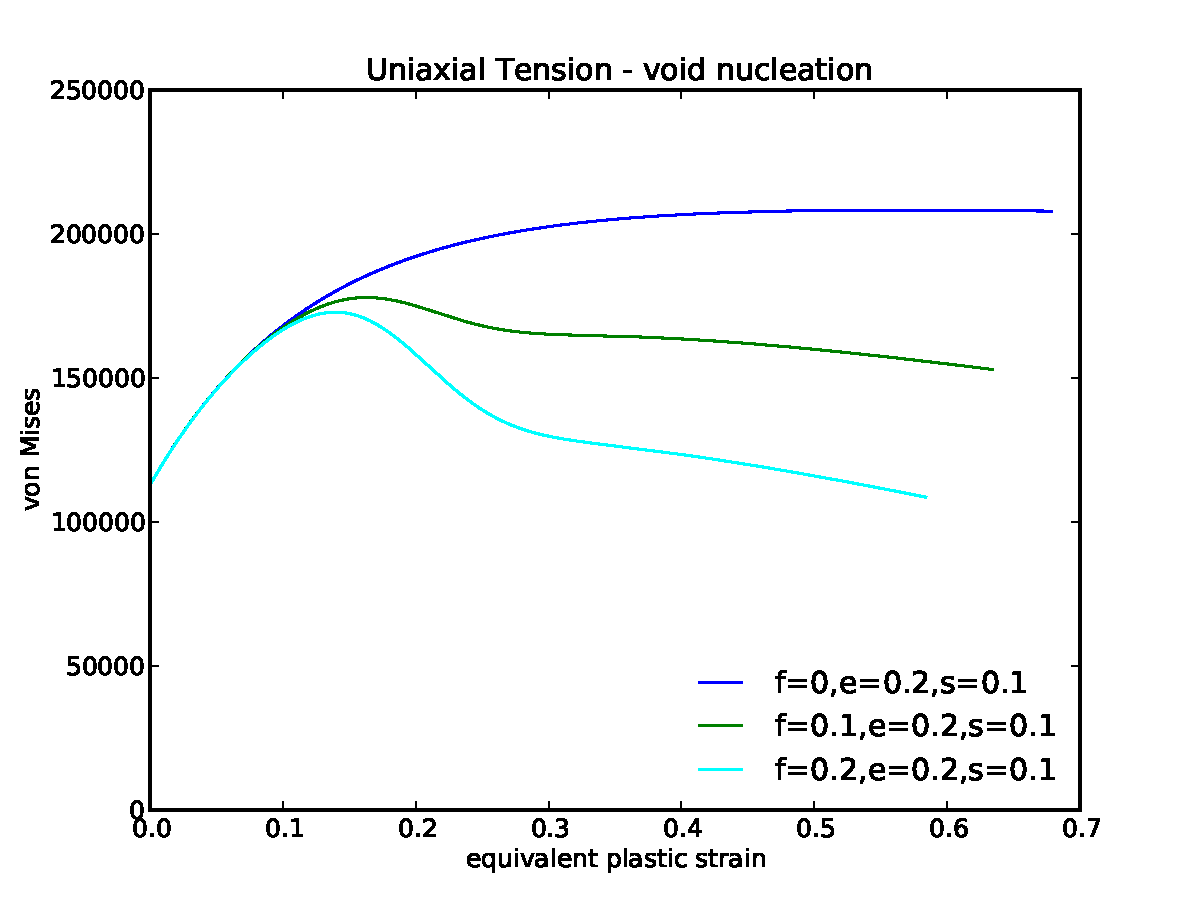
\includegraphics[trim=0mm 0mm 0mm 0
        mm,clip,width=0.5\textwidth]
      {images/stress-strain-tension-nuc.pdf}}~ \subfigure[void volume
      fraction]{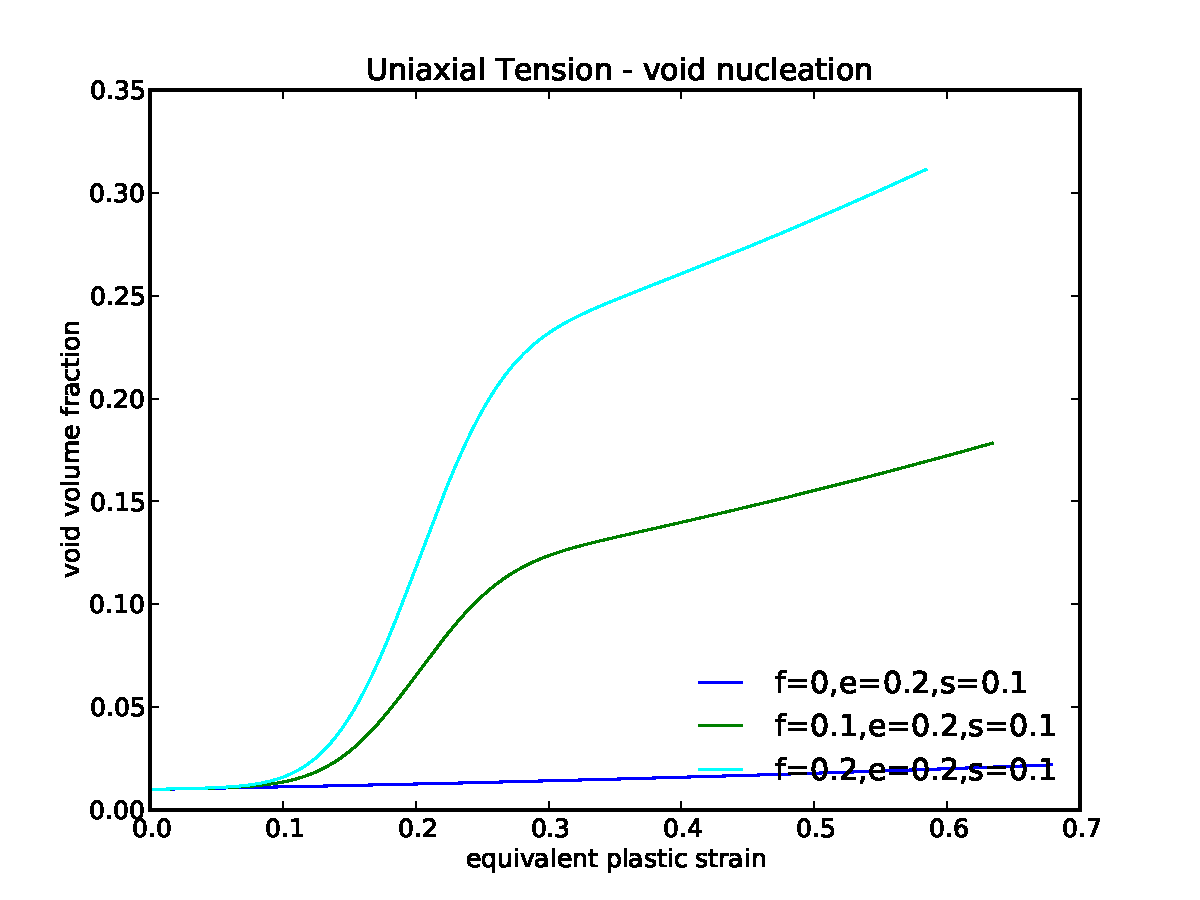
\includegraphics[trim=0mm 0mm 0mm 0
        mm,clip,width=0.5\textwidth]
      {images/void-strain-tension-nuc.pdf}}
    \caption{Von Mises component and void volume fraction plotted
      against equivalent plastic strain. The void nucleation
      parameters have some effect on the response of the
      material point in uniaxial tension.}
    \label{fig:tension-nuc}
  \end{center}
\end{figure}

\section{Simple Shear}
\label{simple-shear}

In this section we investigate the behavior of the two components of
the failure model, specifically the shear dependent void growth and
the void nucleation terms, in the context of simple shear. To test
this problem we use the plasticity parameters developed in the
previous section and study the response of the model to with various
failure parameters. In Figure~\ref{fig:shear-kw} we vary the shear
parameter, $k_{\omega}$, which governs the rate of void growth in
shear dominated states of stress as per \eqref{eq:fg_1}. Observe that
in the extreme case for simple shear $k_{\omega}$ can accelerate void
growth to the point of complete material failure corresponding to the
shear stress component reaching a value of zero.

\begin{figure}[htbp]
  \begin{center}
    \subfigure[stress]{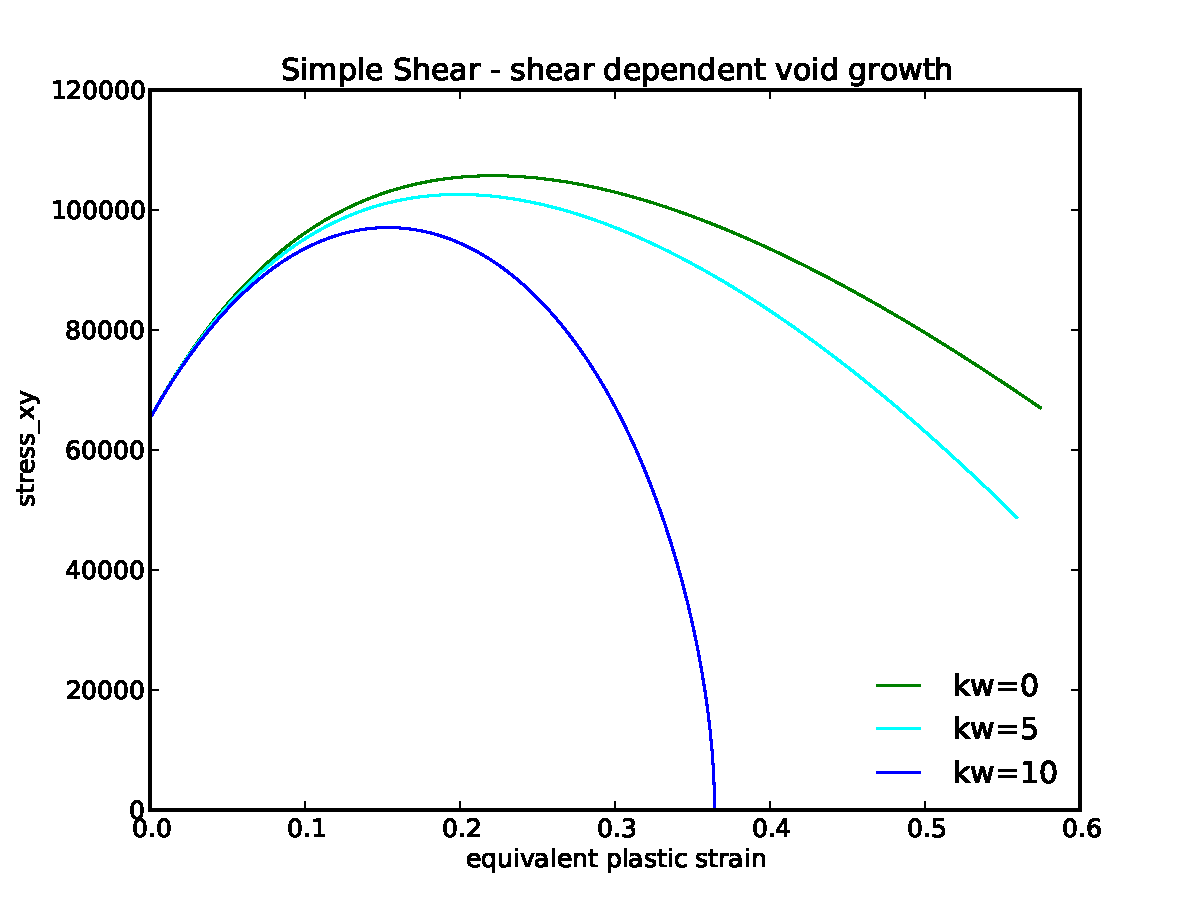
\includegraphics[trim=0mm 0mm 0mm 0
        mm,clip,width=0.5\textwidth]
      {images/stress-strain-shear-kw.pdf}}~ \subfigure[void volume
      fraction]{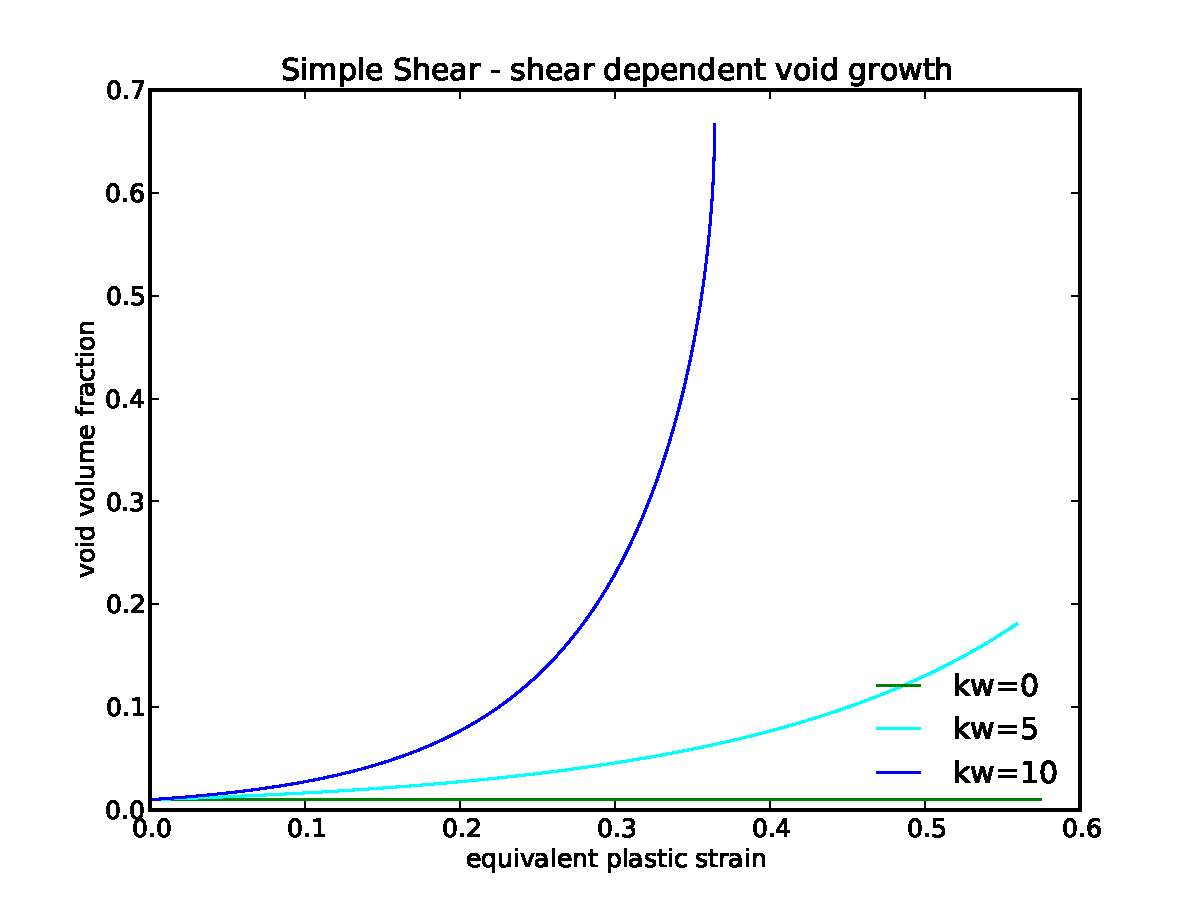
\includegraphics[trim=0mm 0mm 0mm 0
        mm,clip,width=0.5\textwidth]
      {images/void-strain-shear-kw.pdf}}
    \caption{Shear stress component and void volume fraction plotted
      against equivalent plastic strain. The shear void growth
      parameter has a pronounced effect on the response of the
      material point in simple shear.}
    \label{fig:shear-kw}
  \end{center}
\end{figure}

In Figure~\ref{fig:shear-nuc} a set of nucleation parameters are
specified and also evaluated in the simple shear scenario. In this
case the volume fraction of nucleated voids $f_{N}$, is varied, while
the mean value and standard deviation of failure strain, $\epsilon_N$
and $s_N$ respectively, are specified and held constant. Observe that
the shear stress component is somewhat reduced, to a greater extent as
the volume fraction of nucleated voids is increased. Also observe that
the void volume fraction grows by approximately the specified volume
fraction of nucleated voids, in particular, where $f_{N}$ is zero, the
void volume fraction does not deviate from zero.

\begin{figure}[htbp]
  \begin{center}
    \subfigure[stress]{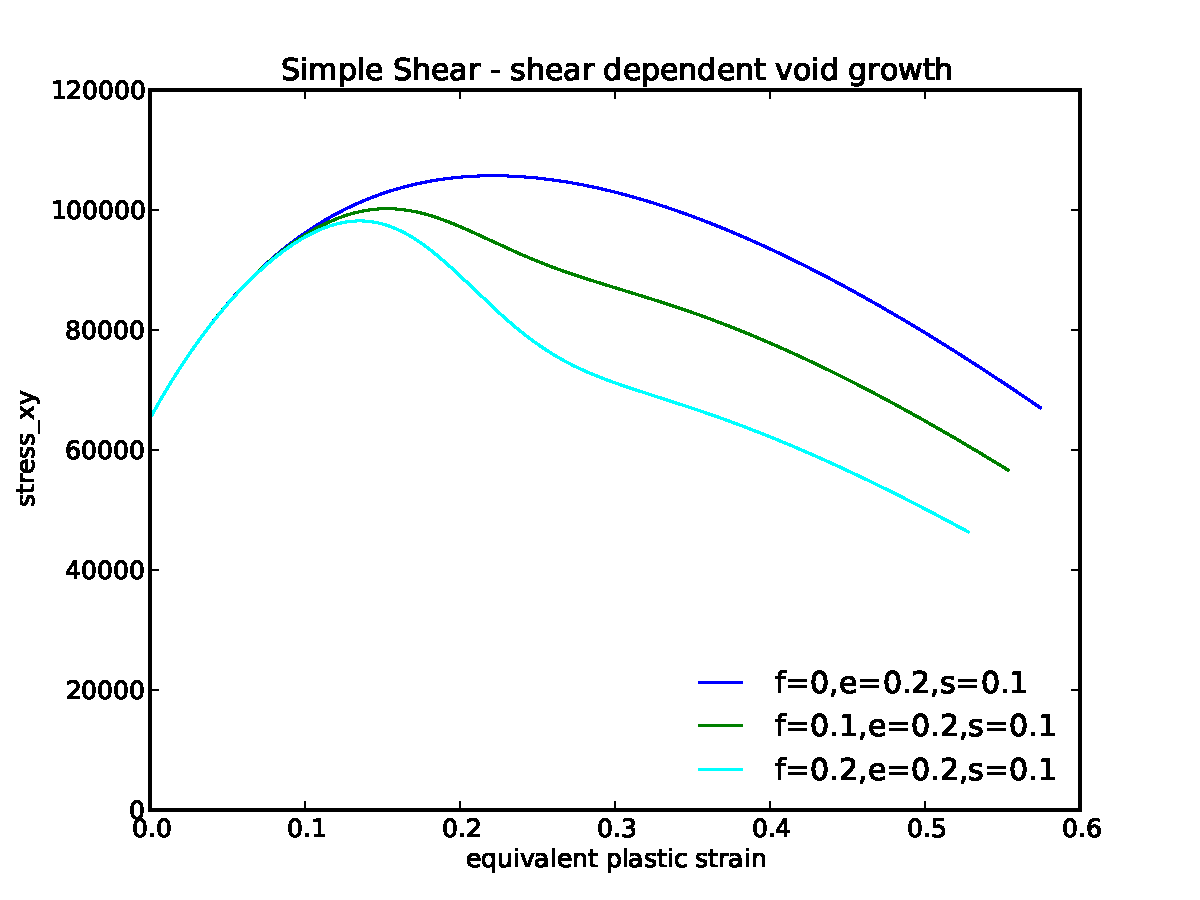
\includegraphics[trim=0mm 0mm 0mm 0
        mm,clip,width=0.5\textwidth]
      {images/stress-strain-shear-nuc.pdf}}~ \subfigure[void volume
      fraction]{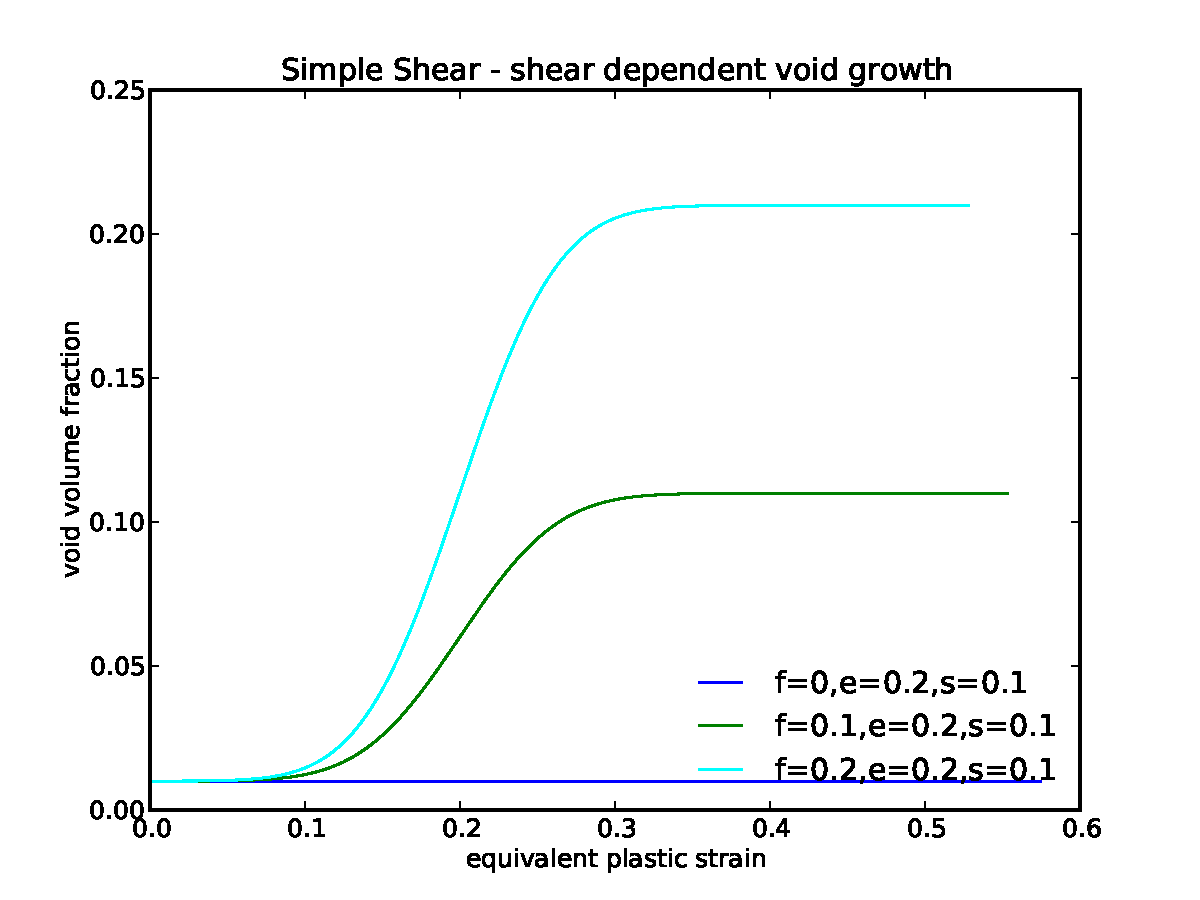
\includegraphics[trim=0mm 0mm 0mm 0
        mm,clip,width=0.5\textwidth]
      {images/void-strain-shear-nuc.pdf}}
    \caption{Shear stress component and void volume fraction plotted
      against equivalent plastic strain. The void nucleation
      parameters have some effect on the response of the
      material point in simple shear.}
    \label{fig:shear-nuc}
  \end{center}
\end{figure}

% Local Variables:
% TeX-master: "GursonModel"
% mode: latex
% mode: flyspell
% End:
